\chapter{Pruebas del funcionamiento del lenguaje }

En esta parte se demuestra código escrito en el lenguaje, y como el compilador y la máquina virtual interactuan con este código fuente.

\section{Programa Factorial}
En este programa se implementaron dos formas para calcular la factorial de un número. Una usando una función recursiva y la otra usando un método secuencial.
A continuación, se presenta el código fuente:
\begin{figure}[htbp]
    \centering
    \begin{lstlisting}
        programa factorial { 
	
    	entero n;
    	entero r[ 2 ];
    	entero l[ 3 ][ 2 ];
    	flotante g[1][1][1];
    	
    	funcion entero factorial (entero num){}{
    		si(num > 0){
    			regresar num * $factorial(num-1);
    		}sino{
    			regresar 1;
    		}
    	}
    
    	
    
    	principal funcion
    	{
    		entero aka,aux,aux2;
    		
    
    	}
    	{
    		n = $factorial(5);
    		imprimir("Factorial de n \n");
    		imprimir(n);
    		aka = 10-n;
    		10 / (-aka) ;
    		aka = 5;
    		aux2 = aka;
    		aux = 1;
    		mientras(aux <= aux2){
    			si (aux2 - aux > 0 ){ 
    				aka = aka * (aux2-aux);
    			}sino{
    				aka = aka * 1;
    			}
    			aux = aux + 1;
    		}
    		imprimir("Factorial Secuencial : ",aka);
    		
    	} 
    
    }

    \end{lstlisting}
    \caption{Código fuente del programa factorial}
    \label{fig:my_label}
\end{figure}
\FloatBarrier

A continuación se muestra su ejecución en consola:
\begin{figure}[htbp]
    \centering
    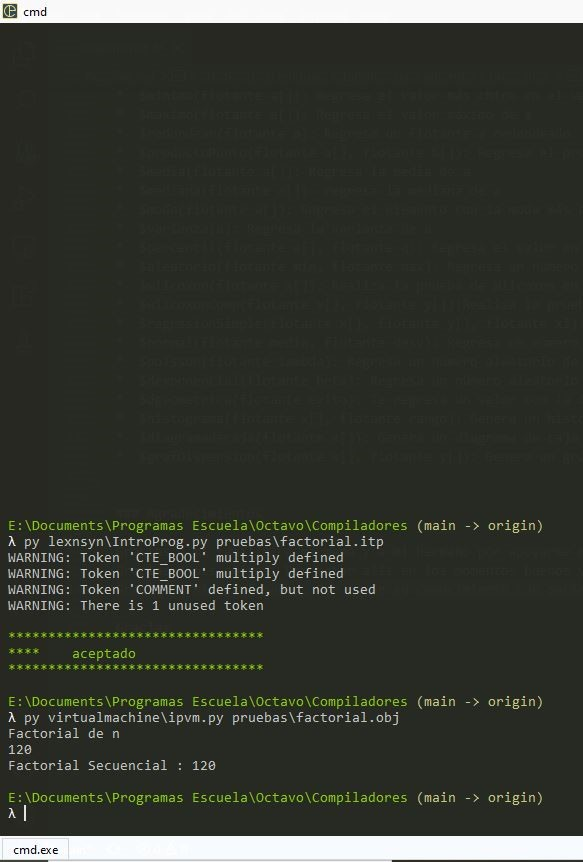
\includegraphics[scale=0.5]{chapters/chapter5/figures/FactorialCorriendo.JPG}
    \caption{El programa factorial compilado y ejecutado}
    \label{fig:my_label}
\end{figure}
\FloatBarrier

\section{Programa Fibonacci}

En este programa se implementaron dos formas para calcular el número n de la serie de Fibonacci. Una usando una función recursiva y la otra usando un método secuencial.
A continuación, se presenta el código fuente:
\begin{figure}[htbp]
    \centering
    \begin{lstlisting}
        programa fibbo { 
    	funcion entero fibbo(entero n){}{
    		si(n == 0){
    			regresar 0;
    		}
    		si(n == 1){
    			regresar 1;
    		}
    		regresar $fibbo(n-1) + $fibbo(n-2);
    	}
    	principal funcion {
    		entero pri,seg,ter,obj,aux;
    	} {	
    		obj = 8;
    		imprimir("fibbo ",$fibbo(obj));
    
    		pri = 0;
    		seg = 1;
    		aux = 1;
    		mientras( aux < obj){
    			ter = pri + seg;
    			pri = seg;
    			seg = ter;
    			aux = aux + 1;
    		}
    		imprimir("Fibbo secuencial : ",ter);
    
    	} 
}

    \end{lstlisting}
    \caption{Código fuente del programa fibbo}
    \label{fig:my_label}
\end{figure}
\FloatBarrier

A continuación se muestra su ejecución en consola:
\begin{figure}[htbp]
    \centering
    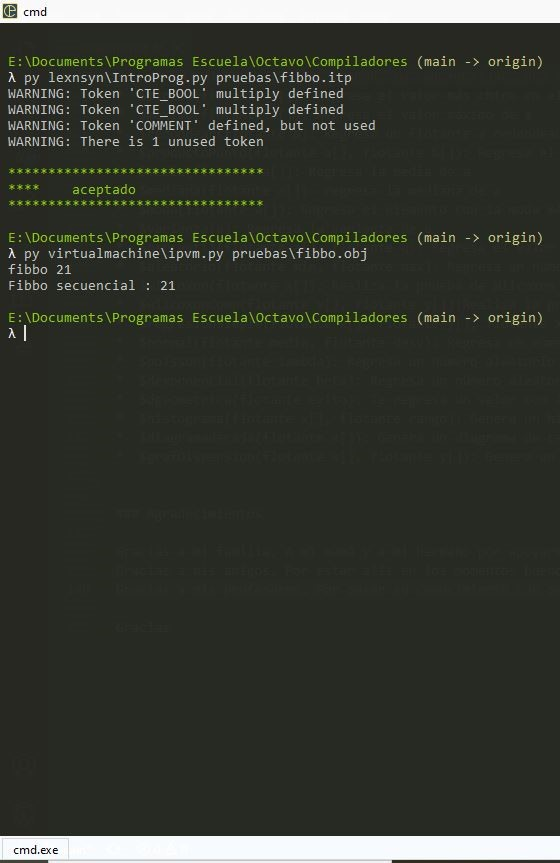
\includegraphics[scale=0.5]{chapters/chapter5/figures/fibbocorriendo.JPG}
    \caption{El programa fibbo compilado y ejecutado}
    \label{fig:my_label}
\end{figure}
\FloatBarrier


\section{Programa Busqueda y organización de arreglo}

En este programa se implementaron una función de búsqueda en un arreglo y un Bubble Sort para organizar un arreglo.
A continuación, se presenta el código fuente:
\begin{figure}[htbp]
    \centering
    \tiny
    \begin{lstlisting}
        programa arraysearchnsort{
            entero a[10];
            funcion vacio imprimirArr(entero a[10]){
                entero x;
            }{
                por(x = 0; x < 10; x = x+1;){
                    imprimir("a[",x,"] = ",a[x]);
                }
            }
        
            funcion vacio encontrar(entero x, entero a[10]){
                entero i,aux,aux2;
                bool loEncontre;
            }{
                imprimir("\n------------------\nBuscando ",x," en el arreglo :");
                $imprimirArr(a);
                imprimir("\n\n");
                aux = -1;
                loEncontre = falso;
                por(i = 0;i < 10;i = i +1;){
                    si(a[i] == x){
                        
                        aux2 = i;
                        i = 10+1;
                        loEncontre = verdadero;
                    }
                }
                si (loEncontre){
                    imprimir("Encontro ",x," en a[",aux2,"]");
                }sino{
                    imprimir("No se encontro el numero");
                }
            }
            principal funcion {
                entero i, j, aux;
            } {
                
                a = [1,5,4,3,2,-7,9,8,6,10];
                $encontrar(4,a);
                $encontrar(-1,a);
                imprimir("Desordenado:\n");
                $imprimirArr(a);
                por(i = 0; i < 10; i = i+1;){
                    por(j = 0; j < 10 -i-1; j = j+1;){
                        si(a[j] > a[j+1]){
                            aux = a[j];
                            a[j] = a[j+1];
                            a[j+1] = aux;
                        }
                    }
                }
                imprimir("\n\nOrdenado:\n");
                $imprimirArr(a);
                imprimir();
            }
        }
    \end{lstlisting}
    \caption{Código fuente del programa arraysearchnsort}
    \label{fig:my_label}
\end{figure}
\FloatBarrier
A continuación se muestra su ejecución en consola:
\begin{figure}[htbp]
    \centering
    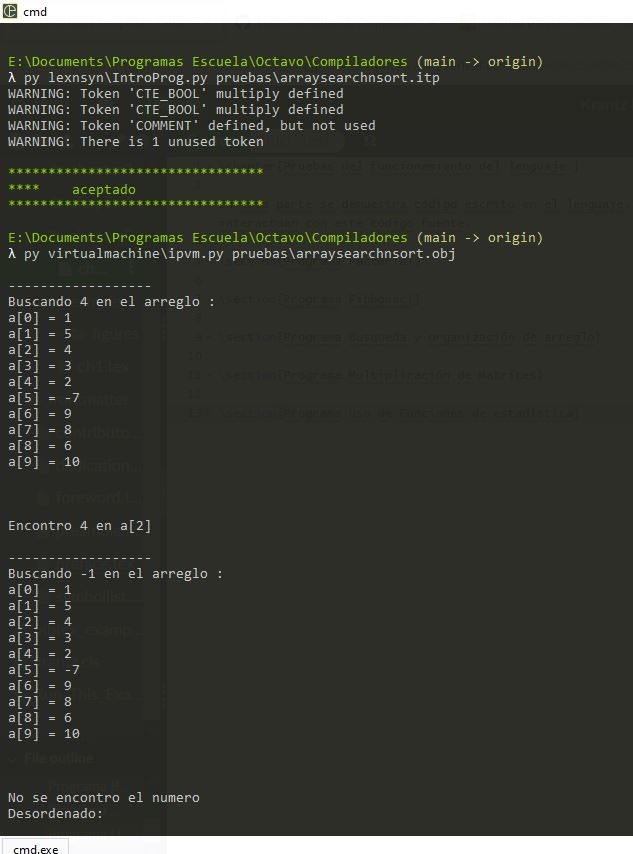
\includegraphics[scale=0.5]{chapters/chapter5/figures/arraycorriendo1.JPG}
    \caption{El Búsqueda y Sort compilado y ejecutado parte 1}
    \label{fig:my_label}
\end{figure}
\FloatBarrier
\begin{figure}[htbp]
    \centering
    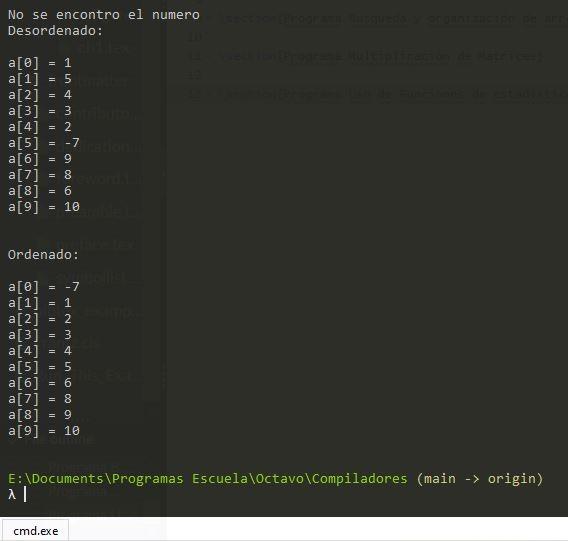
\includegraphics[scale=0.5]{chapters/chapter5/figures/arraycorriendo2.JPG}
    \caption{El Búsqueda y Sort compilado y ejecutado parte 2}
    \label{fig:my_label}
\end{figure}
\FloatBarrier

\section{Programa Multiplicación de Matrices}
En este programa se implemento una función de multiplicación de matrices.
A continuación, se presenta el código fuente:
\begin{figure}[htbp]
    \centering
    \tiny
    \begin{lstlisting}
        programa matmul{
            entero matA[2][3];
            entero matB[3][4];
            entero r1, comun ,c2;
            funcion vacio imprimirMatA(entero a[2][3]){
                entero x,y;
            }{
                por(x = 0; x < 2; x = x+1;){
                    por(y = 0; y < 3; y = y+1;){
                        imprimir("mat[",x ,"][", y,"] = ",a[x][y]);
                    }
                }
                
            }
            funcion vacio imprimirMatB(entero a[3][4]){
                entero x,y;
            }{
                por(x = 0; x < 3; x = x+1;){
                    por(y = 0; y < 4; y = y+1;){
                        imprimir("mat[",x ,"][", y,"] = ",a[x][y]);
                    }
                }
                
            }
        
            funcion vacio imprimirMat(entero a[2][4]){
                entero x,y;
            }{
                por(x = 0; x < 2; x = x+1;){
                    por(y = 0; y < 4; y = y+1;){
                        imprimir("mat[",x ,"][", y,"] = ",a[x][y]);
                    }
                }
                
            }
        
            principal funcion{
                entero matR[2][4];
                entero i,j,k;
            }{
                r1 = 2;
                comun = 3;
                c2 = 4;
                matA = [[1,2,3],[4,5,6]];
                imprimir("Matriz A :");
                $imprimirMatA(matA);
                matB = [[1,2,3,4],[5,6,7,8],[9,10,11,12]];
                imprimir("Matriz B :");
                $imprimirMatB(matB);
                
                por (i = 0; i < r1; i = i+1;) { //Iterar sobre los renglones de la primera matriz
                    por(j = 0; j < c2; j = j +1;){// Iterar sobre las columnas de la segunda matriz
                        matR[i][j] = 0;
                        por(k = 0; k < comun; k = k+1;){ 
                        // Recorer la col/reg para  hacer la multiplicacion
                            matR[i][j] = matR[i][j] + matA[i][k] * matB[k][j]; 
                            //matR[i][j] + matA[R_i][k] * matB[k][C_j]
                        }
                         
                    }
                }
        
                imprimir("Matriz R :");
                $imprimirMat(matR);
            }
        }
    \end{lstlisting}
    \caption{Código fuente del programa matmul}
    \label{fig:my_label}
\end{figure}
\FloatBarrier
A continuación se muestra su ejecución en consola:
\begin{figure}[htbp]
    \centering
    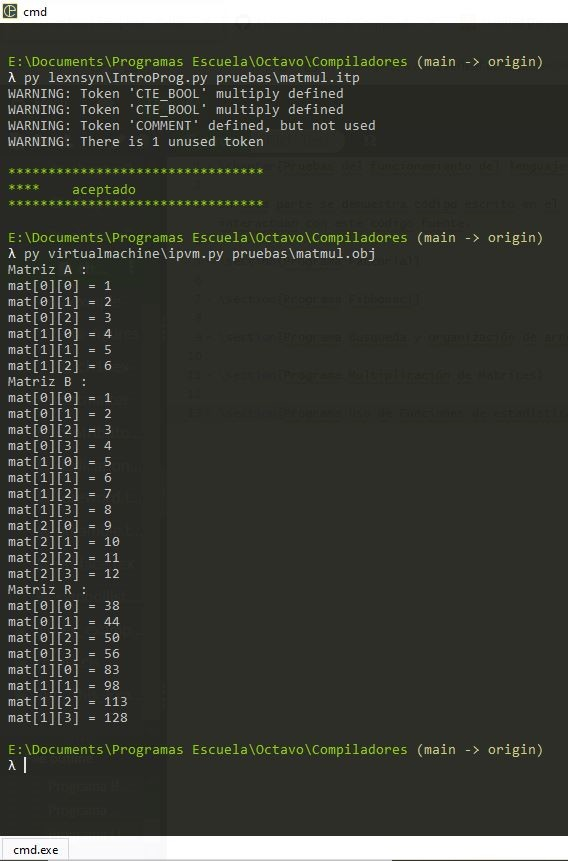
\includegraphics[scale=0.5]{chapters/chapter5/figures/matmulcorriendo.JPG}
    \caption{El matmul compilado y ejecutado}
    \label{fig:my_label}
\end{figure}
\FloatBarrier
\section{Programa Uso de Funciones de estadística}

En este programa se implementaron unas pruebas de Wilcoxon. Se crearon tres arreglos que simulaban muestras las cuales se popularon con números aleatorios pertenecientes a una distribución y se desplego la información básica de cada arreglo. Al final se hicieron unas pruebas  de wilcoxon para probar cual de las muestras se acomodaba mejor.

A continuación, se presenta el código fuente:
\begin{figure}[htbp]
    \centering
    \tiny
    \begin{lstlisting}
        programa pruebasDeWilcoxon{
                // La declaracion de variables
                flotante muestra1[100];
                flotante muestra2[100];
                // Declaracion de funciones
                funcion vacio imprimirDatos( flotante arr[100] ){
                    flotante prom, mod, med;
                }{
                    prom = $media(arr);
                    mod = $moda(arr);
                    med = $mediana(arr);
                    imprimir(" La media de esta distribucion es : ", prom);
                    imprimir(" La mediana de esta distribucion es : ", med);
                    imprimir(" La moda de esta distribucion es : ", mod);
                    imprimir(" El cuartil del 50 de los datos : ", $percentil(arr,50));
                }
                //Funcion principal
                principal funcion {
                    flotante muestra3[100];
                    entero i;
                    flotante p;
                }{
                    por(i = 0; i < 100; i = i+1;){
                        muestra1[i] = $normal(3.5,0.6);
                        muestra2[i] = $dexponencial(4);
                        muestra3[i] = $poisson(2);
                    }
            
                    imprimir("Muestra 1 : Normal");
                    $imprimirDatos(muestra1);
                    imprimir("Muestra 2 : Exponencial");
                    $imprimirDatos(muestra2);
                    imprimir("Muestra 3 : Poisson");
                    $imprimirDatos(muestra3);
            
                    //Pasar una prueba de wilcoxon p > 0.5
                    p = $wilcoxonComp(muestra1,muestra2);
                    imprimir("\n\nMuestra 1 v Muestra 2");
                    si(p > 0.5){
                        imprimir("Muestra 1 es la que mejor representa los datos");
                    }sino{
                        imprimir("Muestra 2 es la que mejor representa los datos");
                    }
            
                    p = $wilcoxonComp(muestra1,muestra3);
                    imprimir("\n\nMuestra 1 v Muestra 3");
                    si(p > 0.5){
                        imprimir("Muestra 1 es la que mejor representa los datos");
                    }sino{
                        imprimir("Muestra 3 es la que mejor representa los datos");
                    }
            
                    p = $wilcoxonComp(muestra3,muestra2);
                    imprimir("\n\nMuestra 3 v Muestra 2");
                    si(p > 0.5){
                        imprimir("Muestra 3 es la que mejor representa los datos");
                    }sino{
                        imprimir("Muestra 2 es la que mejor representa los datos");
                    }
            
                }
            
        }
    \end{lstlisting}
    \caption{Código fuente del programa}
    \label{fig:my_label}
\end{figure}
\FloatBarrier
A continuación se muestra su ejecución en consola:
\begin{figure}[htbp]
    \centering
    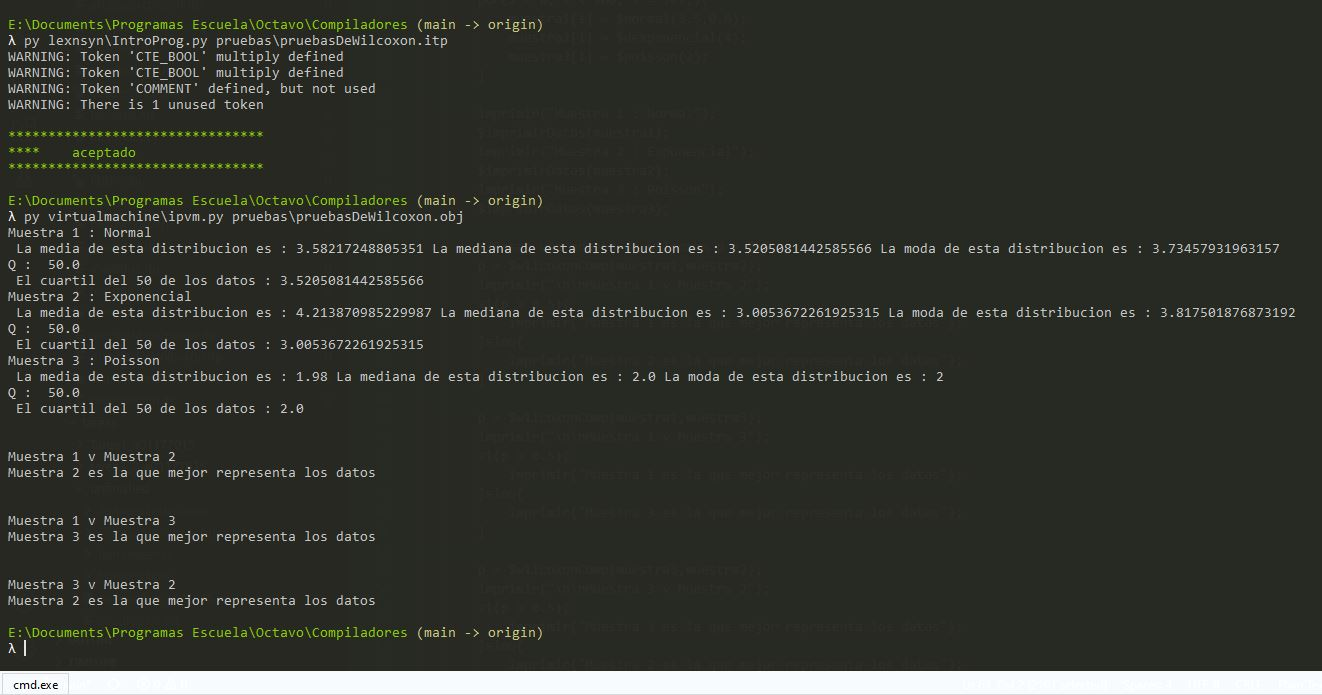
\includegraphics[scale=0.4]{chapters/chapter5/figures/wilcoxCorriendo.JPG}
    \caption{El programa de pruebasDeWilcoxon compilado y ejecutado}
    \label{fig:my_label}
\end{figure}